\documentclass[11pt,xcolor=svgnames]{beamer}
\usepackage{dsfont,natbib,setspace,changepage,multirow}
\mode<presentation>

% replaces beamer foot with simple page number
\setbeamertemplate{navigation symbols}{}
%\setbeamerfont{frametitle}{series=\bfseries}
\setbeamercolor{frametitle}{fg=Black}

\setbeamertemplate{footline}{
   \raisebox{5pt}{\makebox[\paperwidth]{\hfill\makebox[20pt]{\color{gray}\scriptsize\insertframenumber}}}}

\graphicspath{{/Users/mtaddy/Dropbox/inputs/}}
\usepackage{algorithm}
\usepackage{algorithmic}

% colors
\newcommand{\theme}{\color{Maroon}}
\newcommand{\bk}{\color{black}}
\newcommand{\rd}{\color{DarkRed}}
\newcommand{\fg}{\color{ForestGreen}}
\newcommand{\bl}{\color{blue}}
\newcommand{\gr}{\color{black!50}}
\newcommand{\sg}{\color{DarkSlateGray}}
\newcommand{\nv}{\color{Navy}}
\setbeamercolor{itemize item}{fg=gray}

% common math markups
\newcommand{\bs}[1]{\boldsymbol{#1}}
\newcommand{\mc}[1]{\mathcal{#1}}
\newcommand{\mr}[1]{\mathrm{#1}}
\newcommand{\bm}[1]{\mathbf{#1}}
\newcommand{\ds}[1]{\mathds{#1}}
\newcommand{\indep}{\perp\!\!\!\perp}
\def\plus{\texttt{+}}
\def\minus{\texttt{-}}

% spacing and style shorthand
\setstretch{1.1}

\begin{document}

\setcounter{page}{0}
{ \usebackgroundtemplate{\includegraphics[height=\paperheight]{phoenix}}
\begin{frame}[plain]
\begin{center}

{\bf \LARGE \theme }

{\bf \Large  Big Data and Bayesian Nonparametrics

\vskip .25cm
{\theme Example:} Empirical Bayesian Forests}

\vskip 2cm
Matt Taddy,  Chicago Booth


\vskip .25cm
{\texttt{faculty.chicagobooth.edu/matt.taddy/research}}

\end{center}
\end{frame} }


\begin{frame}

{\bf Big Data}

\vskip .5cm
{\nv The sample sizes are enormous.}
\begin{itemize}
\item we'll see 12, w21 and 200 million today.  
\item Data can't fit in memory, or even storage, on a single machine.
\item Our familiar MCMC algorithms take too long.
\end{itemize}

\vskip .25cm
{\nv The data are super weird.  }
\begin{itemize}
\item Internet transaction data distributions have a big spike at zero and spikes at other discrete values (e.g., 1 or \$99).
\item Big tails  that matter.
\item We cannot  write down believable models.
\end{itemize}

\end{frame}

\begin{frame}

Both `Big' and `Strange' beg for nonparametrics.

\vskip .5cm
In usual BNP you {\it model} a complex generative process with flexible priors, then apply that model directly in prediction and inference.
\[
\text{e.g.,~~~}y = f(\bm{x}) + \epsilon,~~\text{or~even~just}~~f(y|\bm{x})
\]
However averaging over all of the nuisance parameters we introduce to be `flexible' is a hard computational problem.

\vskip .5cm
\hfill {\theme Can we do scalable BNP?}
\end{frame}

\begin{frame}

Frequentists are great at finding simple procedures {\gr\small (e.g. $[\bm{X}'\bm{X}]^{-1}\bm{X}'y$)\!} and  showing that they will `work' regardless of the true DGP.

\hfill{\gr \small (DGP = Data Generating Process)~~~~~~~}

\vskip .5cm
This is classical `distribution free' nonparametrics.

\vskip .15cm
1: Find some statistic that is useful regardless of DGP.

\vskip .15cm
2: Derive the distribution for this stat under minimal assumptions.

\vskip .5cm
Practitioners apply the simple stat and feel happy that it will work.

% {\gr No need to re-model the underlying DGP each time, and you \\don't need to have a PhD in Bayesian Statistics to apply the ideas.}

\vskip .5cm\hfill
{\theme Can we Bayesians provide something like this?}

\end{frame}

\begin{frame}

{\bf Distribution free Bayesian nonparametrics}

\vskip .5cm
{Find some {\it statistic of the DGP} that you care about.}
\vskip .1cm
\begin{itemize}
\item Derive it from first principles, e.g. moment conditions.
\item Or a statistic could be an algorithm that we know works.
\end{itemize}
\vskip .1cm
Call this statistic $\mathcal{S}(g)$ where $g(\bm{z})$ is the DGP (e.g., for $\bm{z} = [\bm{x},y]$).

\vskip .5cm
Then you write down a flexible  model for the DGP $g$, and study properties of the posterior on $\mathcal{S}(g)$ induced by the posterior over $g$.

\end{frame}

\begin{frame}

{\bf A flexible model for the DGP}

\vskip .5cm  Let's go back to Ferguson '73 and a multinomial sampling model:

\begin{equation*}
g(\bm{z}) = \frac{1}{|\bs{\theta}|}\sum_{l=1}^L \theta_l \ds{1}{[\bm{z} =
\bs{\zeta}_l]}, \end{equation*}$\bs{\mc{Z}} = \{\bs{\zeta}_1 \dots
\bs{\zeta}_L\}$ is the {\it fixed} support of the DGP and $\theta_l \stackrel{iid}{\sim} \mr{Exp}(a)$.

\vskip .25cm
After observing $\bm{Z} = \{\bm{z}_1 \ldots \bm{z}_n\}$, posterior has $\theta_l \sim \mr{Exp}(a\!+\!\ds{1}_{\bs{\zeta}_l \in \bm{Z}})$. {\gr (say every $\bm{z}_i$ is unique)}.

\vskip .5cm
Taking $a \to 0$ leads to $\mr{p}(\theta_l = 0) = 1$ for $\bs{\zeta}_l \notin \bm{Z}$.

\vskip .1cm
So the posterior has $g(\bm{z}) = \tfrac{1}{|\bs{\theta}|}
\sum_{l=1}^L \theta_l \ds{1}{[\bm{z} =
\bm{z}_l]}$ with $\theta_i \sim \mr{Exp}(1)$.

\vskip .5cm\hfill
{\theme This is just the Bayesian bootstrap.}

\vskip -.5cm
\end{frame}

\begin{frame}

{\bf {\theme Example: } Ordinary Least Squares}

\vskip .5cm
The {\it population} OLS projection is a posterior functional
\begin{equation*}
\bs{\beta} = (\bm{X}'\bs{\Theta}\bm{X})^{-1}  \bm{X}'\bs{\Theta}\bm{y}
\end{equation*}
where $\bs{\Theta} = \mr{diag}(\bs{\theta})$.  
{\theme This is a random variable \bk (sample via BB).}


\vskip .5cm We can derive posterior moments for a first-order approx
\[
\bs{\tilde \beta} = [\bm{X}'\bm{X}]^{-1}\bm{X}'y + 
\nabla \bs{\beta}\big |_{\bs{\theta}=\bm{1}} (\bs{\theta} - \bm{1})
\]
e.g., $\mr{var}(\bs{\tilde \beta}) \approx (\bm{X}^{\prime}\bm{X})^{-1}\bm{X}^{\prime}\mr{diag}(\bm{e})^2\bm{X}^{\prime}(\bm{X}^{\prime}\bm{X})^{-1}$, where $e_i  = y_i - \bm{x}_i'\bs{\hat\beta}$.

\vskip .5cm{\gr \hfill
 See Lancaster 2003 or Poirier 2011.}

\end{frame}


\begin{frame}


{\bf {\theme Example:} Decision Trees}

\vskip .5cm
Trees are great: nonlinearity, deep interactions, heteroskedasticity.

\begin{center}
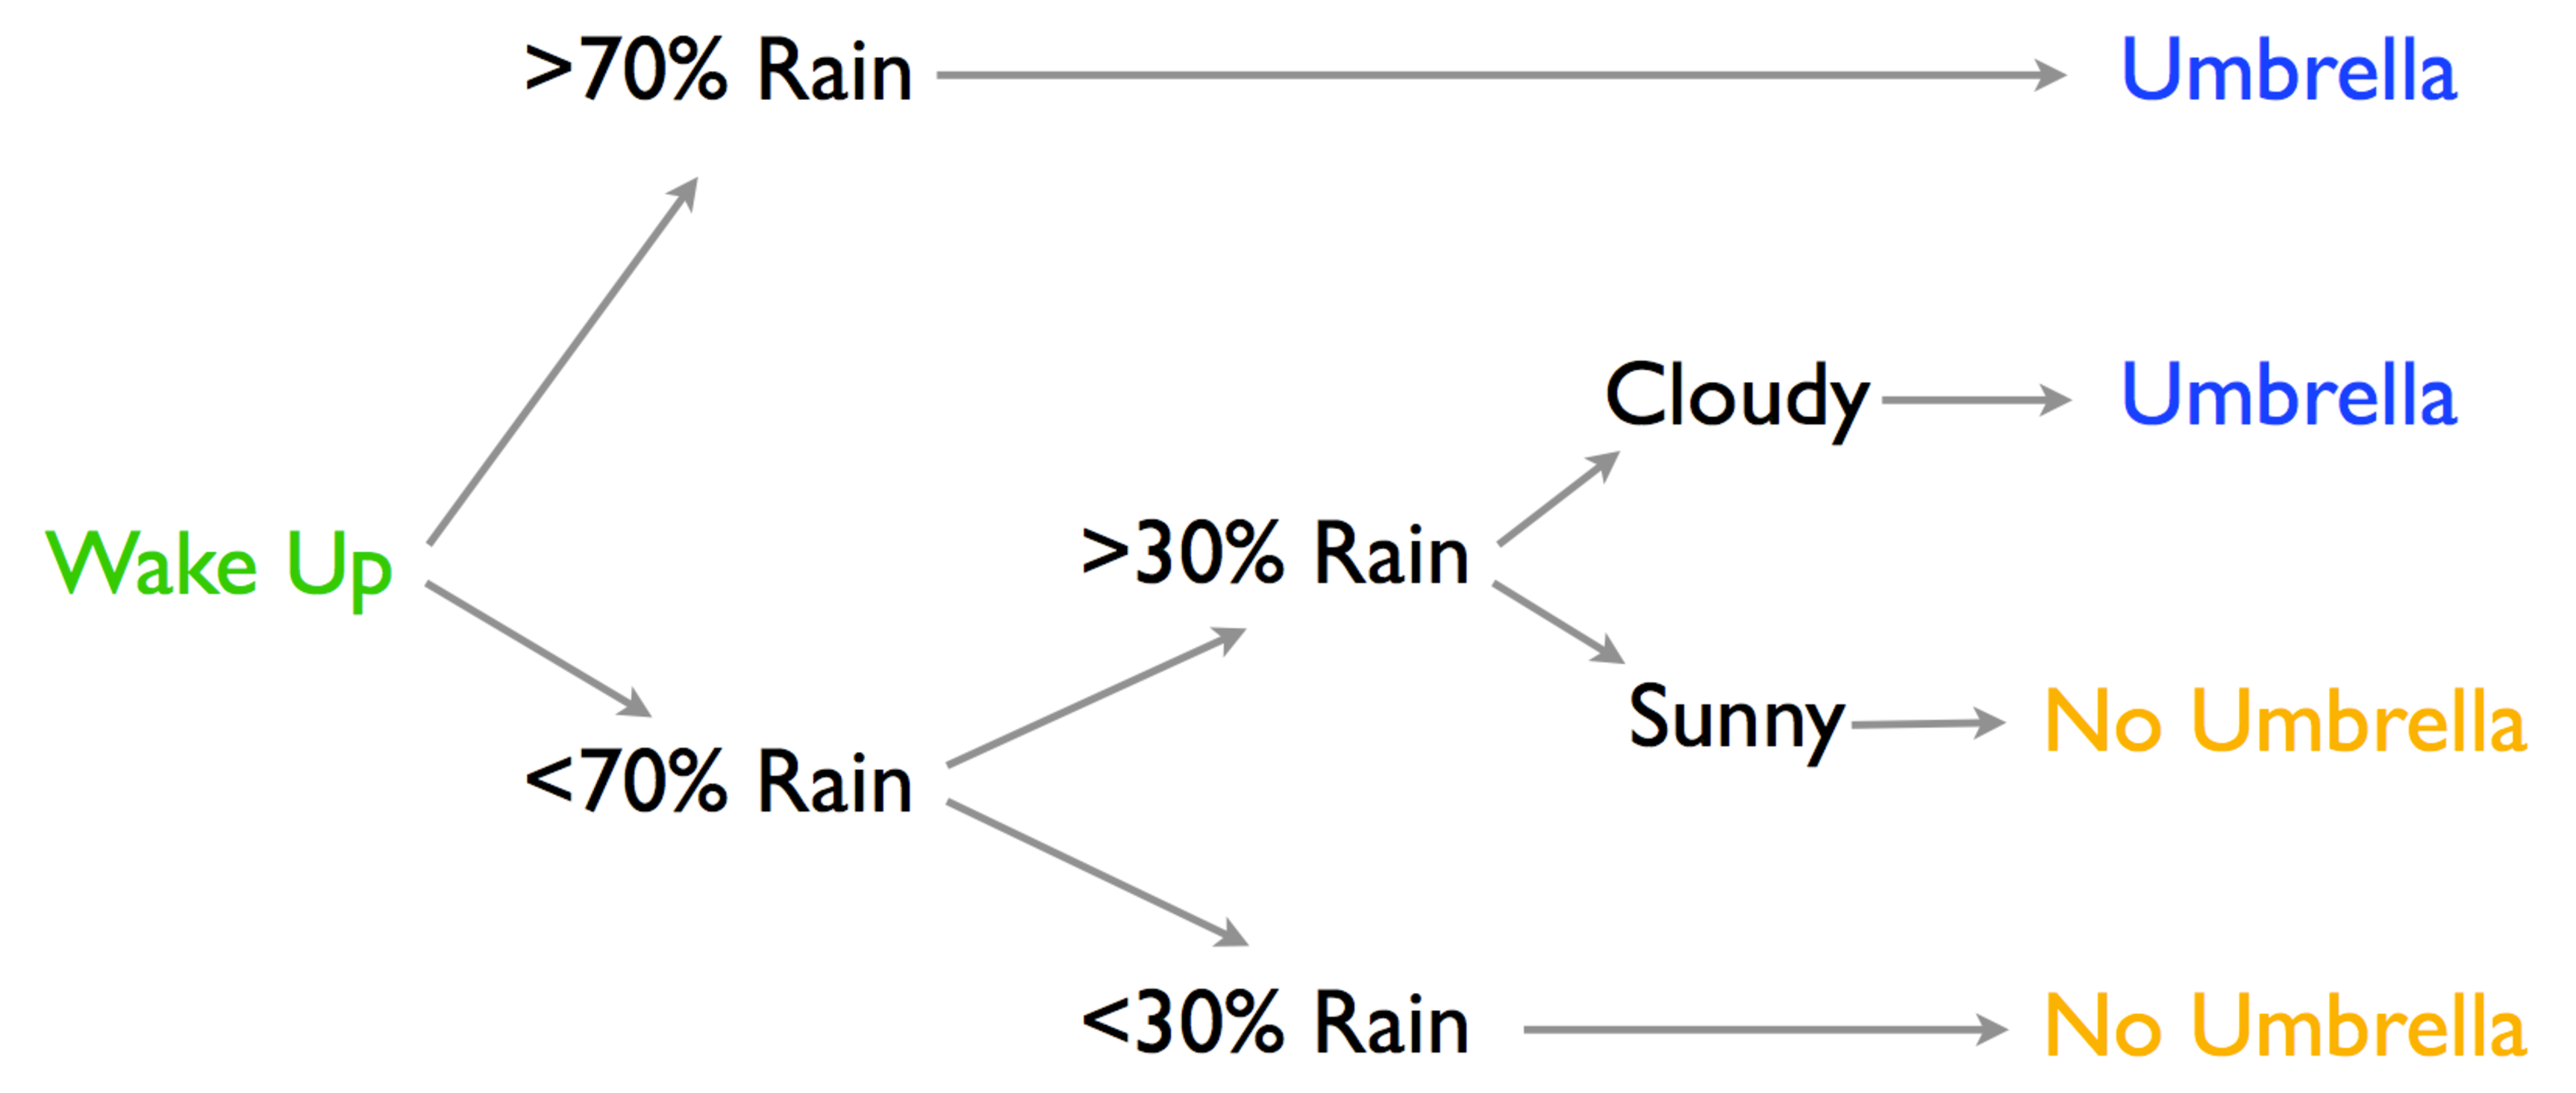
\includegraphics[width=4in]{../graphs/umbrella}
\end{center}

The `optimal' decision tree is a statistic we care about {\gr (s.w.c.a)}.


\end{frame}


\begin{frame}


{\bf CART} fits a tree by greedily growing with optimal splits.

\vskip .5cm
Given {\nv parent} node $\{\bm{x}_i,y_i\}_{i=1}^n$, the optimal split
finds $x_{ij}$ so that 
\[
\mathrm{left}(x_{ij}):\{\bm{x}_k,y_k:~x_{kj} \leq x_{ij}\}
\text{~~and~~}\mathrm{right}(x_{ij}):\{\bm{x}_k,y_k:~x_{kj} > x_{ij}\}
\]
{\nv child} sets are as homogeneous in response $y$ as possible.


e.g., a regression tree recursively splits to  minimize 
\[
|\bs{\theta}|\sigma^2(x, \bs{\theta} ) = \sum_{k \in \mathrm{left}(x)} \theta_k (y_k - \mu_{\mathrm{left}(x)})^2 + \sum_{k \in \mathrm{right}(x)} \theta_k (y_k - \mu_{\mathrm{right}(x)})^2
\]
where $\theta_k$ are observation weights  and $\displaystyle\mu_{\mathrm{c}(x)} = \frac{1}{|\bs{\theta}_{\mathrm{c}(x)}|} \sum_{k \in \mathrm{c}(x)} \theta_ky_k$.

\vskip .5cm{\theme
If population-CART would predict well, then it's a s.w.c.a.}



\end{frame}


\begin{frame}[fragile]

{\bf \theme Bayesian Forests: \bk Sample the posterior for CART trees}

\vskip .25cm
For $b=1 \dots B$: \\
   ~~~~~~~~~~$\bullet$ draw $\boldsymbol{\theta}^b \stackrel{iid}{\sim} \mathrm{Exp}(\mathbf{1})$
   \\
   ~~~~~~~~~~$\bullet$ run weighted-sample CART to get $\mathcal{T}_b = \mathcal{T}(\boldsymbol{\theta}^b)$
 
\vskip .5cm\small 
~~~~~~~~~~~~~~~~~~~~~{\it one tree~~~~~~~~~~~~~~~~~~~~~~~~~~~~~~~~~~posterior mean}\\

\includegraphics[height=1.75in]{../../bayesian-forest/graphs/MCtreedraw}   
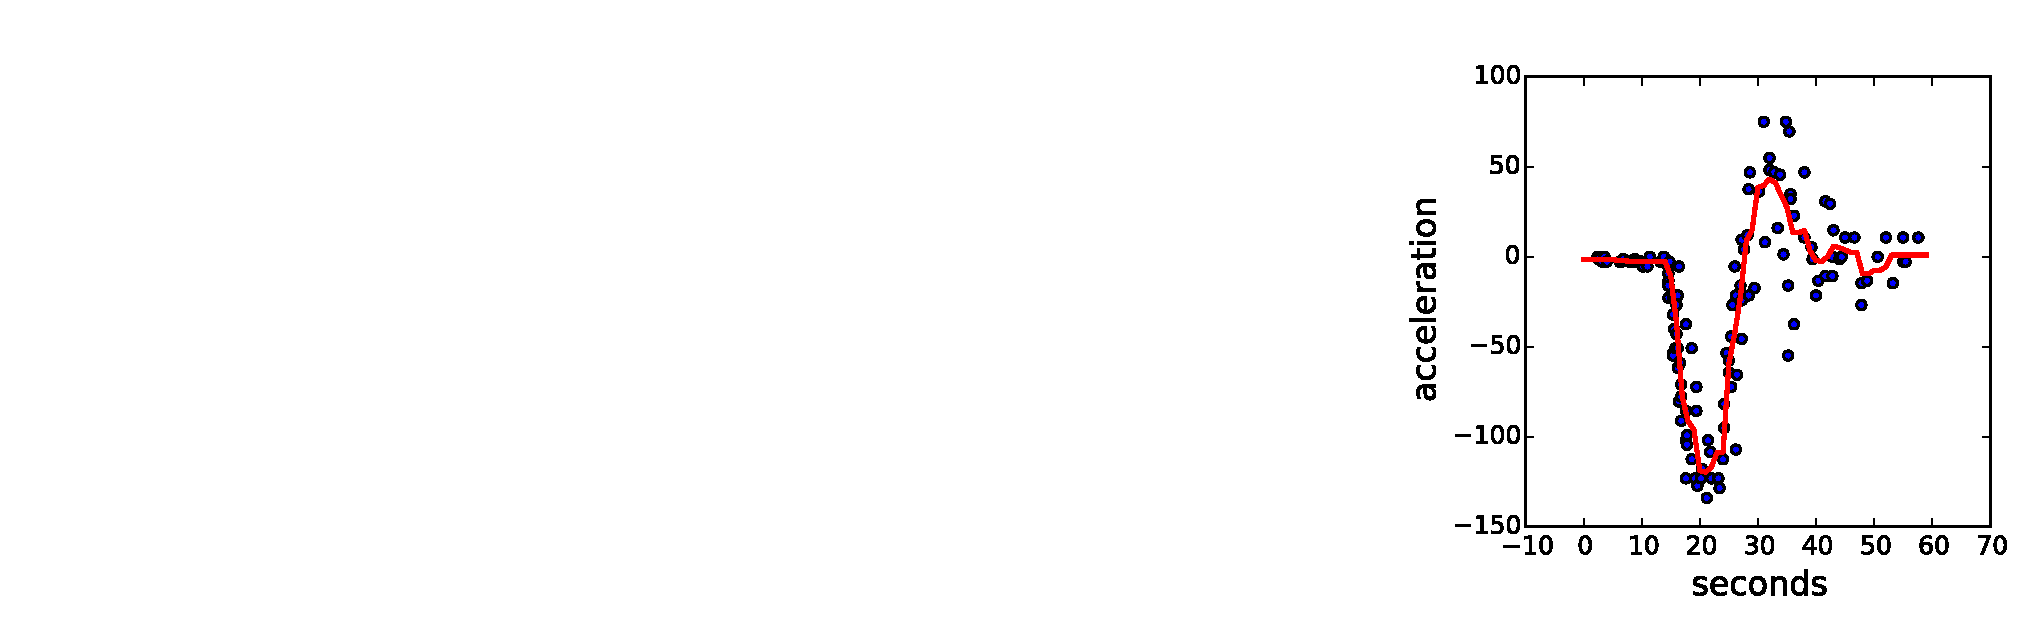
\includegraphics[height=1.75in]{../../bayesian-forest/graphs/MCbforest}   

\vskip .25cm
This is {\it very similar} to a random forest.  So, RFs $\approx$ posterior over trees.
\vskip -.5cm

\end{frame}



\begin{frame}

{\bf Theoretical {\theme trunk} stability}

\vskip .5cm

Given forests as a posterior, 
we can start talking about {\it variance}.

\vskip .1cm
As in simple OLS, look at the posterior for 1st order approx.
\[
\sigma^2(x,\bs{\theta}) \approx \sigma^2(x,\boldsymbol{1}) + \nabla \sigma^2\big |_{\boldsymbol{\theta}=\mathbf{1}} (\boldsymbol{\theta} - \boldsymbol{1}) =  \frac{1}{n}\sum_i \theta_i \left[y_i - \bar{y}_i(x)\right]^2
\]
with $\bar y_i (x)$ the sample mean in $i$'s node when splitting on $x$.

\vskip .1cm
Based on this approx, we can say that for data at a given node, 
\begin{equation*}\theme
\mathrm{p}\left(\text{optimal split matches sample CART}\right) \gtrsim 1 - \frac{p}{\sqrt{n}} e^{-n},
\end{equation*}
with $p$ split locations and $n$ observations.  

\vskip .5cm{\nv Things are pretty stable, until they aren't: as the tree grows,  node sizes get smaller and chance of a non-optimal split multiplies.}

\end{frame}

\begin{frame}

{\bf California Housing Data}


\vskip .5cm

20k observations on median home prices in zip codes.

\vskip .5cm

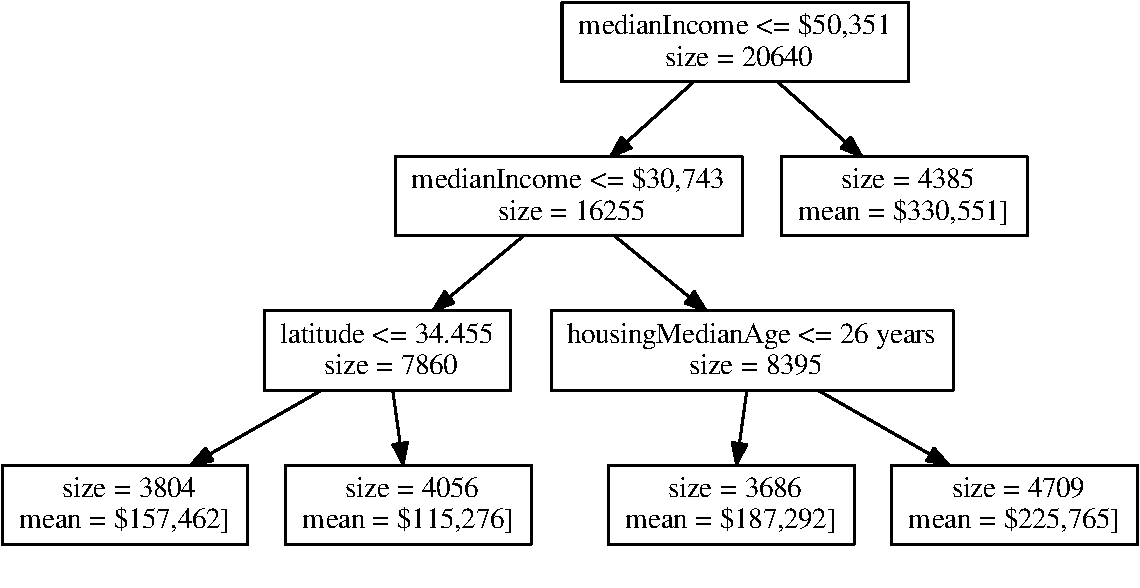
\includegraphics[width=\textwidth]{../../bayesian-forest/graphs/ca_trunk}

\vskip .5cm
\hfill Above is the trunk you get setting min-leaf-size of 3500.

\end{frame}

\begin{frame}

\begin{columns}

\begin{column}{2.15in}
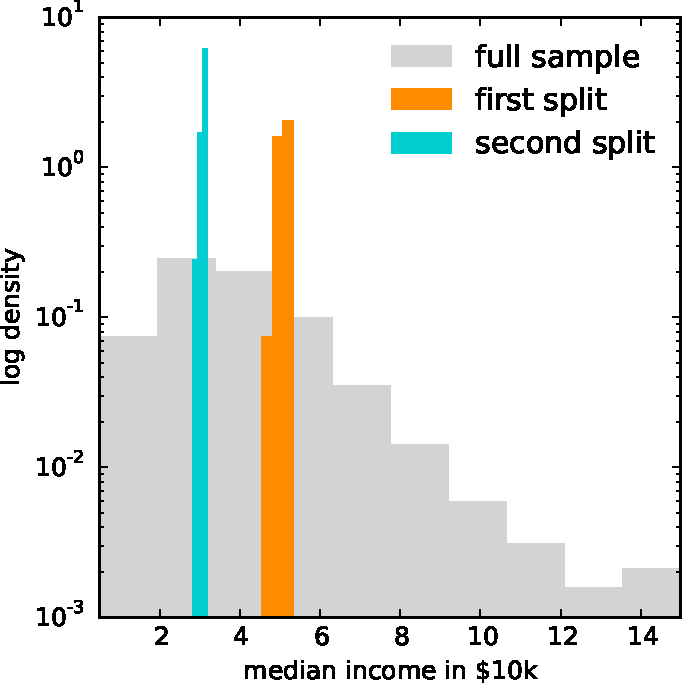
\includegraphics[width=2.5in]{../../bayesian-forest/graphs/ca_splits}
\end{column}

\begin{column}{2in}
\begin{itemize}
\item sample tree occurs 62\% \\of the time.  
\vskip .5cm
\item 90\% of  trees split on income twice, \\and then latitude. 

\vskip .5cm
\item 100\% of trees have 1st 2 splits on median income.  
\end{itemize}
\end{column}

\end{columns}


\vskip 1cm
~~~~Empirically and theoretically: trees are stable, at the trunk.
\vskip -1cm

\end{frame}

\begin{frame}


Forests are expensive when data is too big to fit in memory.

Subsampling forests 
lead to a big drop in performance.

\vskip .5cm
{\bf Empirical Bayesian Forests ({\theme EBF}):}

\vskip .25cm
\begin{itemize}
\item fit a single tree to a shallow {\nv trunk}.  
\item Use this as a mapper to direct full data to each {\nv branch}.  
\item Fit a full  forest on the smaller branch datasets.
\end{itemize}

\vskip .25cm
This is classic Empirical Bayes: fix higher levels in a {\it hierarchical model}, and direct your machinery\texttt{+}data at learning the hard bits.

\end{frame}

\begin{frame}


Since the trunks are all the same for each tree in a full forest,
our EBF looks nearly the same at a fraction of computational cost.

\begin{center}
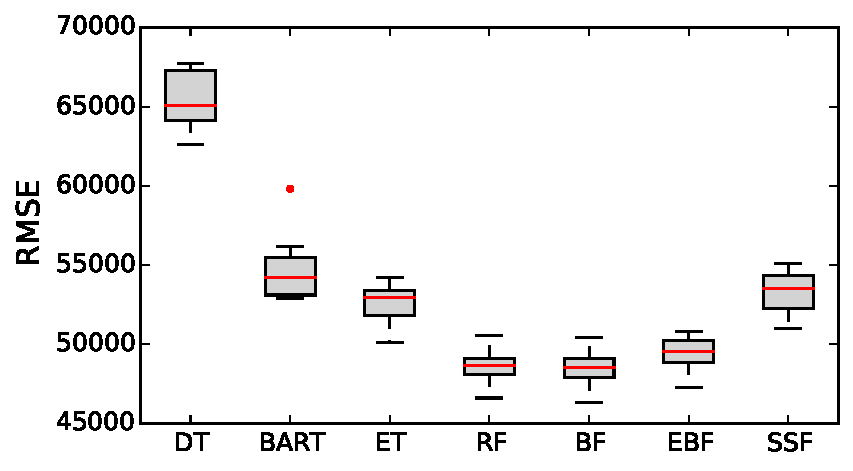
\includegraphics[width=.85\textwidth]{../../bayesian-forest/graphs/ca_rmse}
\end{center}

Here EBF and BF give nearly the same results.  {\it SSF does not.}


\end{frame}


\begin{frame}

{\bf EBFs work all over the place}

\vskip .5cm
\begin{minipage}{0.5\linewidth}
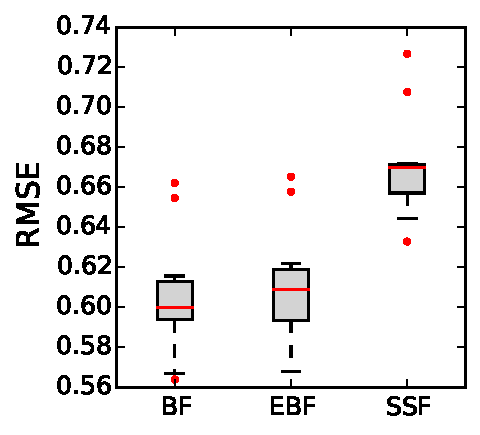
\includegraphics[width=\textwidth]{../graphs/wine}
\end{minipage}
~~
\begin{minipage}{0.4\linewidth}
{\footnotesize
\begin{tabular}{c c | l}
$\overline{\text{RMSE}}$  & \% WTB & \\
\cline{1-2}\rule{0pt}{3ex} 
0.5905 &  0.0 & BF \\
0.5953 &  0.8 & EBF \\
0.6607 & 11.9 & SSF \\
0.7648 & 29.5 & DT \\
\end{tabular}}
\end{minipage}

\vskip .5cm
\hfill Predicting wine rating from chemical profile

\end{frame}


\begin{frame}

{\bf EBFs work all over the place}

\vskip .5cm
\begin{minipage}{0.5\linewidth}
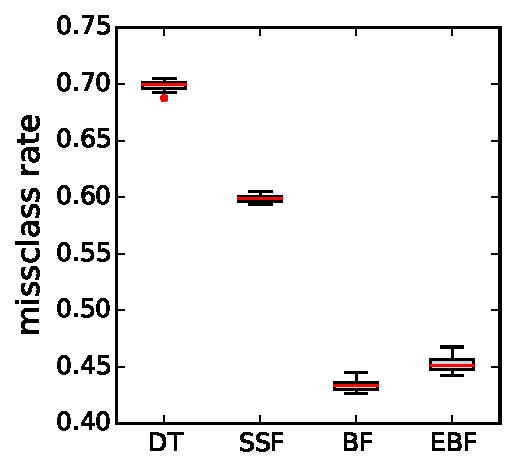
\includegraphics[width=\textwidth]{../graphs/beer}
\end{minipage}
~~
\begin{minipage}{0.4\linewidth}
{\footnotesize
\begin{tabular}{c c | l}
$\overline{\text{MCR}}$  & \% WTB & \\
\cline{1-2}\rule{0pt}{3ex} 
0.4341 &  0.0 & BF \\
0.4531 &  4.4 & EBF \\
0.5989 & 38.0 & SSF \\
0.6979 & 60.8 & DT \\
\end{tabular}}
\end{minipage}

\vskip .5cm
\hfill or beer choice from demographics

\end{frame}

\begin{frame}

{\bf Choosing the trunk depth}


\vskip .5cm
Distributed computing perspective: {\theme fix only as deep as you must!}

\vskip .1cm
How big is each machine? Make that your branch size.

\vskip .75cm
{\small
\begin{tabular}{c | c c c | c c c | c c c}
& \multicolumn{3}{l|}{CA housing} & \multicolumn{3}{l|}{Wine} &\multicolumn{3}{l}{Beer} \\
\cline{2-10} \rule{0pt}{3ex} 
\!\!\!\!\!\!{\it Min Leaf Size in $10^3$} & 6 & 3 & 1.5 & 2  & 1 & 0.5 & 20 & 10 & 5\\
\!\!\!\!\!\!{\it \% Worse Than Best} & \!1.6 & \!2.4 & \!4.3 & \!0.3 & \!0.8 & \!2.2 & \!1.0 & \!4.4 & \!7.6 
\end{tabular}}

\vskip .5cm
Still, open questions:  e.g., more trees vs shallower trunk?

% \vskip .25cm
% A key point: we {\theme do not} think that EBFs are better than forests fit to all the data.  But EBFs allow you to fit to {\nv much more data} in less time without hurting performance too much.


\end{frame}

\begin{frame}


{\bf \theme EBFs at EBay: \bk predicting Bad Buyer Experiences}

\vskip .5cm
A BBE could be receiving something that is `significantly not as described',
or shipping delays, or any of many other problems.

\vskip .5cm
The models are updated frequently, and  information\\ about $\mathrm{p}(\text{BBE})$
is an input to search rankings  and more.

\vskip .5cm The best thing to improve predictions is more data.  \\With millions of daily transactions, there's little limit on data.


% \vskip .25cm
% {\nv Big Data axiom}: more data beats fancy model.

\end{frame}

\begin{frame}

{\bf EBFs at EBay}

\vskip .5cm
Random forest runs take too long on full data.

\vskip .25cm
Subsampling led to a noticeable and big drop in performance.

\vskip .5cm
So: EBFs!
\begin{itemize}
\item trunk can be fit in distribution using Spark \texttt{MLLib}.
\item this trunk  acts as a sorting function to map observations \\to 
separate locations corresponding to each branch.
\item Forests are then fit on a machine for each branch.  
\end{itemize}



\end{frame}

\begin{frame}

{\bf EBFs at EBay}

\vskip .5cm

On 12 million transactions,  EBF with 32 branches yields a\\ 1.3\% drop in misclassification over the SSF alternatives.  

\vskip .5cm 
Putting it into production requires some careful engineering, \\but this really is a very simple algorithm.  {\theme Big gain, little pain.} 

\vskip .5cm
A key point:  EBFs are not inherently `better' than forests fit to all of the data.  But EBFs can be fit to {\nv more data} in less time.


\end{frame}


\begin{frame}

\vskip .5cm
{\bf Efficient Big Data analysis}

\vskip .25cm
To cut computation without hurting performance, we need to think about what portions of the `model' are {\theme hard} or {\nv easy} to learn.

\vskip .25cm
Once we figure this out,  we can use a little bit of the data to\\ learn the easy stuff and direct our full data at the hard stuff.

\vskip .25cm
I believe that this is the future for Big Data.

\vskip .75cm
{\bf Big Data and distribution free BNP}

\vskip .25cm I think about BNP as a way to analyze (and improve) algorithms.  

Decouple  action/prediction from the full generative process model.

\vskip 1cm
\hfill \huge \theme \bf thanks!

\end{frame}



\end{document}






























